\subsection{Standard Chi-squared distribution}

The pdf of the Chi-squared distribution in the standard basis is

\begin{align}\label{eq:chi2_pdf}
	\mathcal{C}_X(x, k) &= \frac{1}{2^{k/2}\Gamma(k/2)}  x^{k/2 -1} \exp(-x/2) \\
	&= \frac{1}{x}\exp \left[(k/2)\log(x) - x/2 - \log(2^{k/2}\Gamma(k/2))\right]
\end{align} 

with $h(x)=\frac{1}{x}$, $\phi(x) = (\log(x), x), w = k/2$ and $Z(k) = \log(2^{k/2}\Gamma(k/2))$.

\subsubsection{Laplace approximation of the standard Chi-squared distribution}

\begin{align*}
\text{log-pdf: } &(k/2-1)\log(x) - x/2 - \log(2^{k/2}\Gamma(k/2)) \\
\text{1st derivative: }&  \frac{k/2-1}{x} - \frac{1}{2} \\
\text{mode: }&  \frac{k/2-1}{x} - \frac{1}{2} = 0 \Leftrightarrow x = k-2\\
\text{2nd derivative: }&  -\frac{k/2-1}{x^2}\\
\text{insert mode: }& -\frac{k/2-1}{(k-2)^2} = -\frac{(k-2)}{2(k-2)^2}\\
\text{invert and times -1: }&\sigma^2 = 2(k-2)
\end{align*}

\subsection{Log-Transformed Chi-squared distribution}

we transform the distribution with $g(x) = \log(x)$, i.e. $x(y) = g^{-1}(x) = \exp(y)$. The new pdf becomes

\begin{align}
	\mathcal{C}_{Y\_\log}(y,k) &= \frac{1}{2^{k/2}\Gamma(k/2)}  \exp(y)^{k/2 -1} \exp(-\exp(y)/2) \cdot \exp(y) \\
	&= \frac{1}{2^{k/2}\Gamma(k/2)}  \exp(y)^{k/2} \exp(-\exp(y)/2)
	&= \exp\left[\frac{k}{2}y - \frac{\exp(y)}{x} - \log(2^{k/2}\Gamma(k/2))\right]
\end{align}

meaning $h(y) = 1, \phi(y) =(y, \exp(y)), \eta=(k/2)$ and $Z(k) =  \log(2^{k/2}\Gamma(k/2))$. 

\subsubsection{Laplace approximation of the log-transformed Chi-squared distribution}

\begin{align*}
\text{log-pdf: } &\frac{k}{2}y - \frac{\exp(y)}{2} - \log(2^{k/2}\Gamma(k/2)) \\
\text{1st derivative: }&  \frac{k}{2} - \frac{\exp(y)}{2} \\
\text{mode: }& k/2 - \frac{\exp(y)}{2} = 0 \Leftrightarrow y = \log(k)\\
\text{2nd derivative: }&  -\frac{\exp(y)}{2}\\
\text{insert mode: }& -\frac{\exp(y)}{2} = -k/2\\
\text{invert and times -1: }&\sigma^2 = 2/k
\end{align*}

which yields the Laplace Approximation $q(y) = \mathcal{N}(y; \mu= \log(k), \sigma^2 = 2/k)$.

\subsubsection{The Bridge for log-transform}

\begin{align}
	\mu &= \log(k) \\
	\sigma^2 &= 2/k \\
	k &= \exp(\mu)
\end{align}

\begin{figure}[!htb]
	\centering
	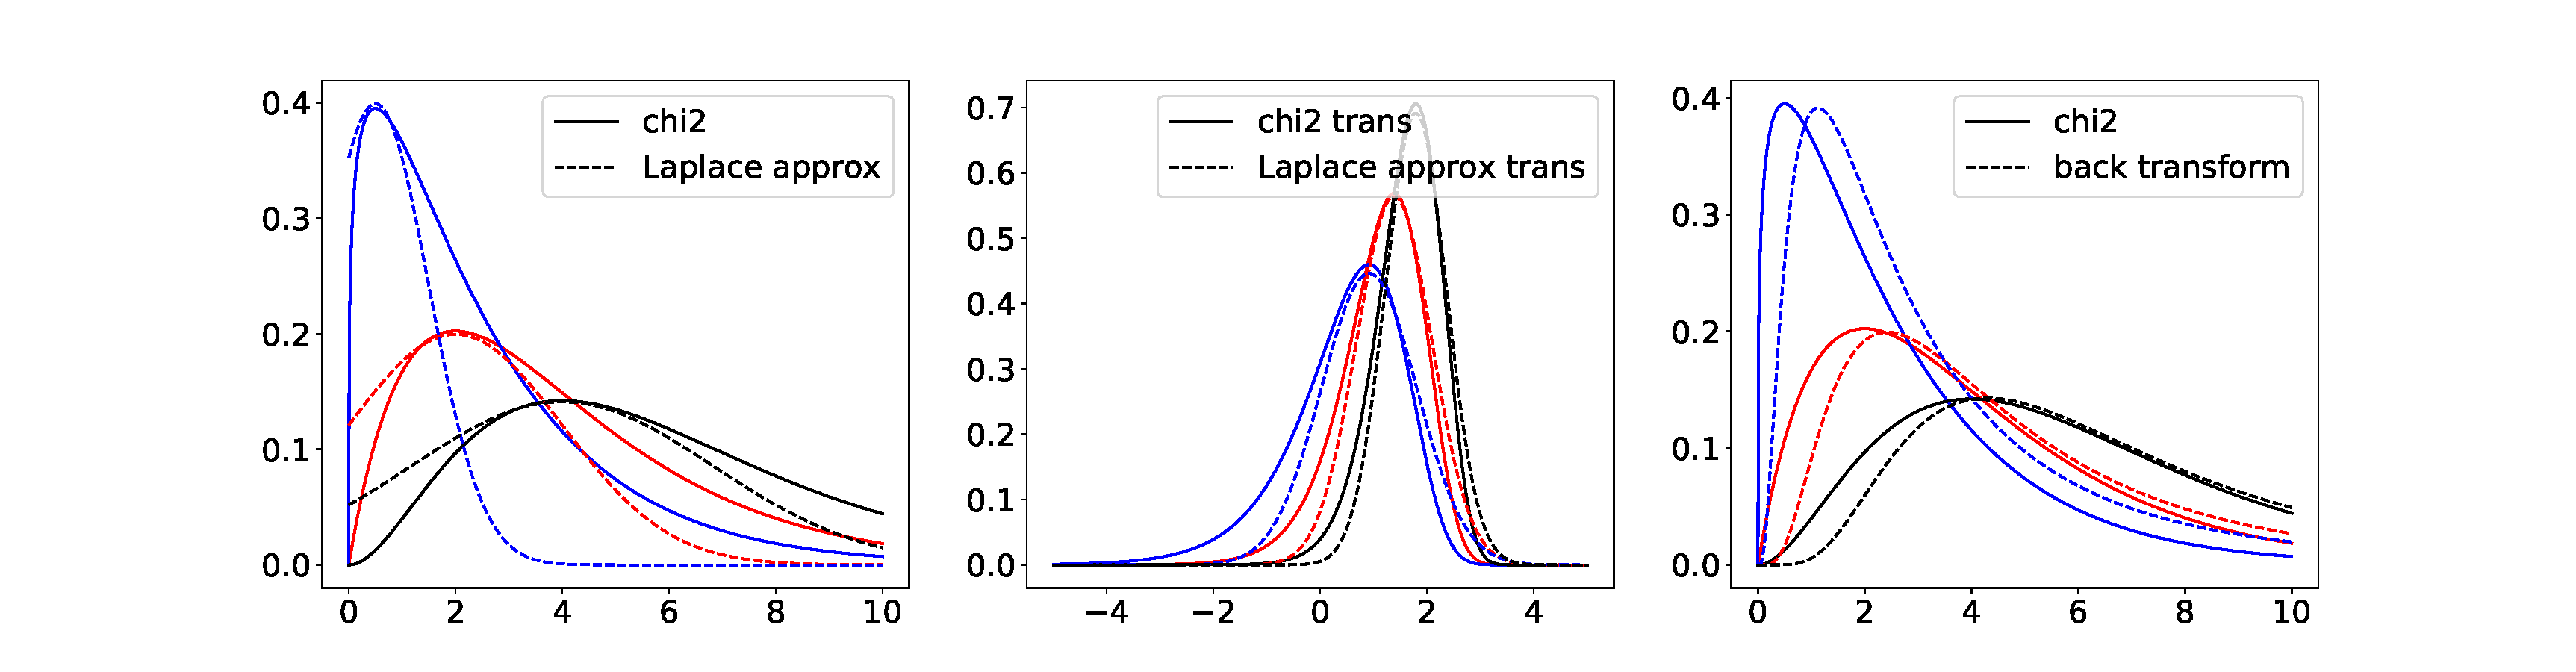
\includegraphics[width=\textwidth]{figures/chi2_playground_log.pdf}
	\caption{chi2 comparison log transform}
	\label{fig:chi2_log_comparison}
\end{figure}

\subsection{Sqrt-Transformed Chi-squared distribution}

we transform the distribution with $g(x) = \sqrt{x}$, i.e. $x(y) = g^{-1}(x) = y^2$. The new pdf becomes

TODO: nasty transform as in beginning.

\begin{align}
\mathcal{C}_{Y_sqrt}(y,k) &= \frac{1}{2^{k/2}\Gamma(k/2)}  y^{2(k/2 -1)} \exp(-y^2/2) \cdot 2y \\
		 &= \frac{1}{2^{k/2}\Gamma(k/2)}  y^{k} \exp(-\frac{y^2}{2}) \\
		 &= \exp \left[k\log(y) - \frac{y^2}{2} - \log(2^{k/2}\Gamma(k/2))\right]
\end{align}


meaning $h(y) = 1, \phi(y)=(\log(y), y^2), w=(k, 1/2)$ and $Z(k) =  \log(2^{k/2}\Gamma(k/2))$. 

\subsubsection{Laplace approximation of the sqrt-transformed Chi-squared distribution}

\begin{align*}
\text{log-pdf: } &(k\log(x) - \frac{x^2}{2} - \log(2^{k/2}\Gamma(k/2)) \\
\text{1st derivative: }&  \frac{k}{x} -x \\
\text{mode: }& \frac{k}{x} -x = 0 \Leftrightarrow x = \sqrt{k}\\
\text{2nd derivative: }&  -\frac{k}{x^2} - 1\\
\text{insert mode: }& -\frac{k}{k}-1\\
\text{invert and times -1: }&\sigma^2 = 1/2
\end{align*}

\subsubsection{The Bridge for sqrt-transform}

\begin{align}
\mu &= \sqrt{k} \\
\sigma^2 &= 1/2 \\
k &= \mu^2
\end{align}

TODO:THE BRIDGE BACK LOOKS A BIT WEIRD\\

\begin{figure}[!htb]
	\centering
	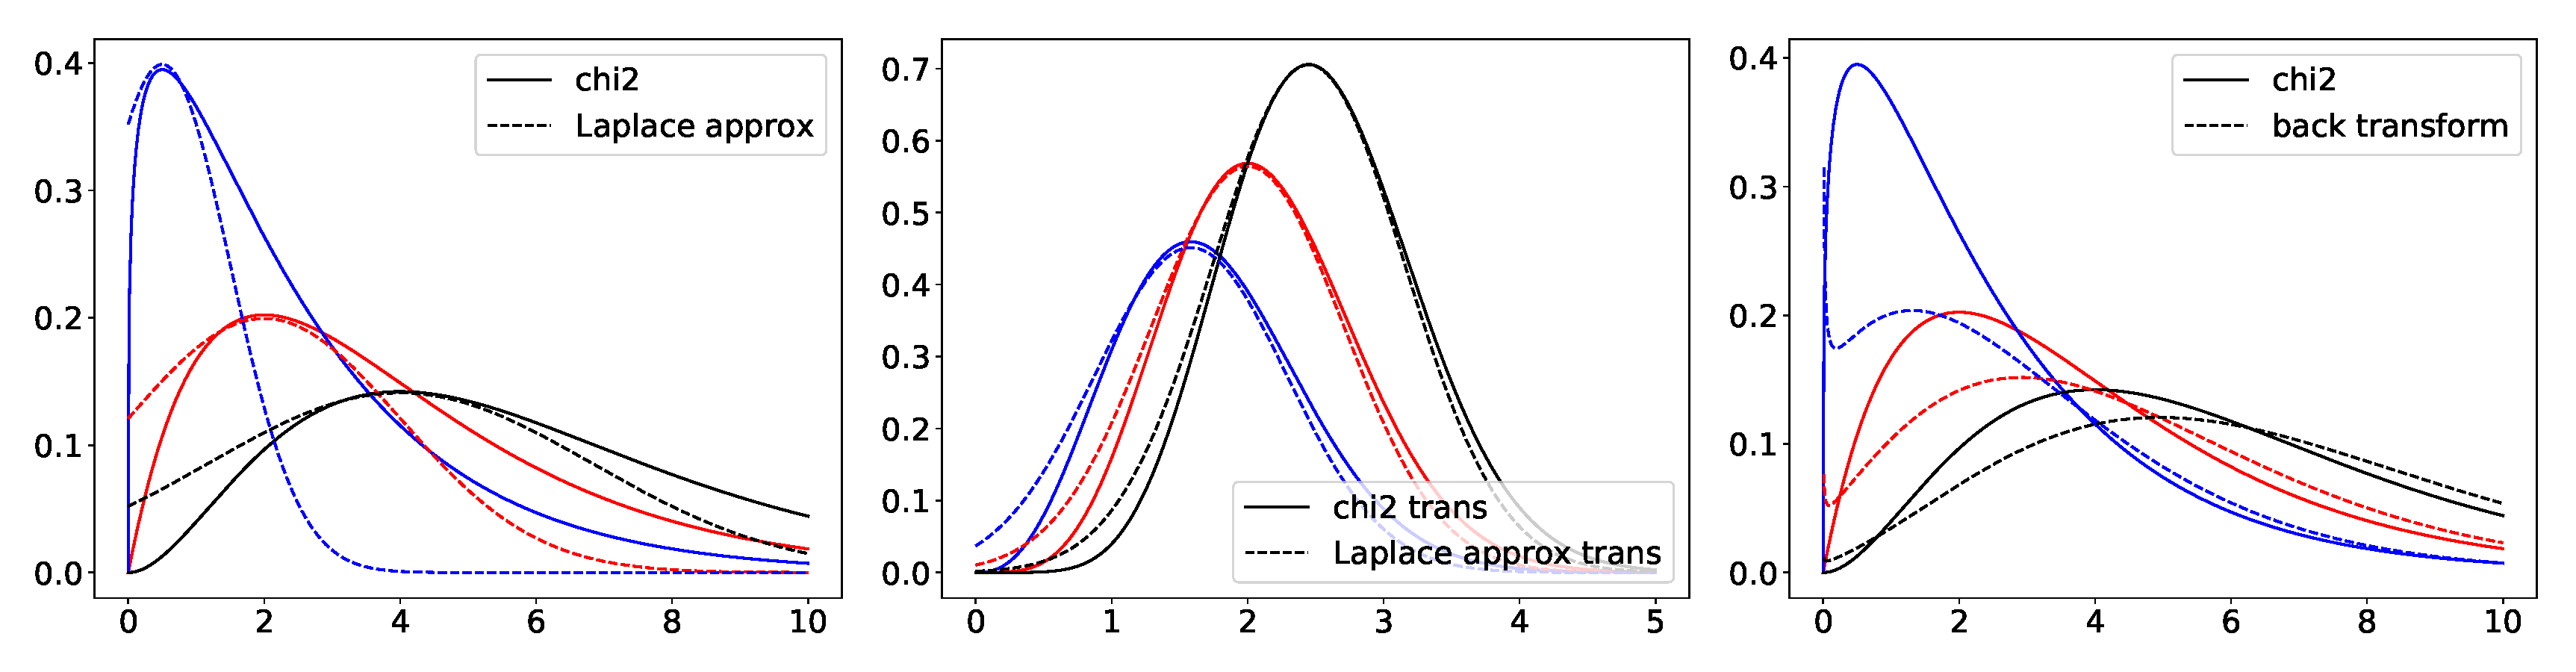
\includegraphics[width=\textwidth]{figures/chi2_playground_sqrt.pdf}
	\caption{chi2 sqrt comparison}
	\label{fig:chi2_sqrt_comparison}
\end{figure}